\documentclass[11pt,french,a4paper]{report}
\usepackage[utf8]{inputenc}
\usepackage[french]{babel}
\usepackage[T1]{fontenc}

\usepackage[left=2cm,right=2cm,top=2cm,bottom=2cm]{geometry}
\geometry{a4paper}
\usepackage{graphicx} 
\usepackage{fancyhdr}
\pagestyle{fancy}
\usepackage{lastpage}


\fancyhead[L]{\includegraphics[scale=00.3]{../../logo/logo_um.PNG}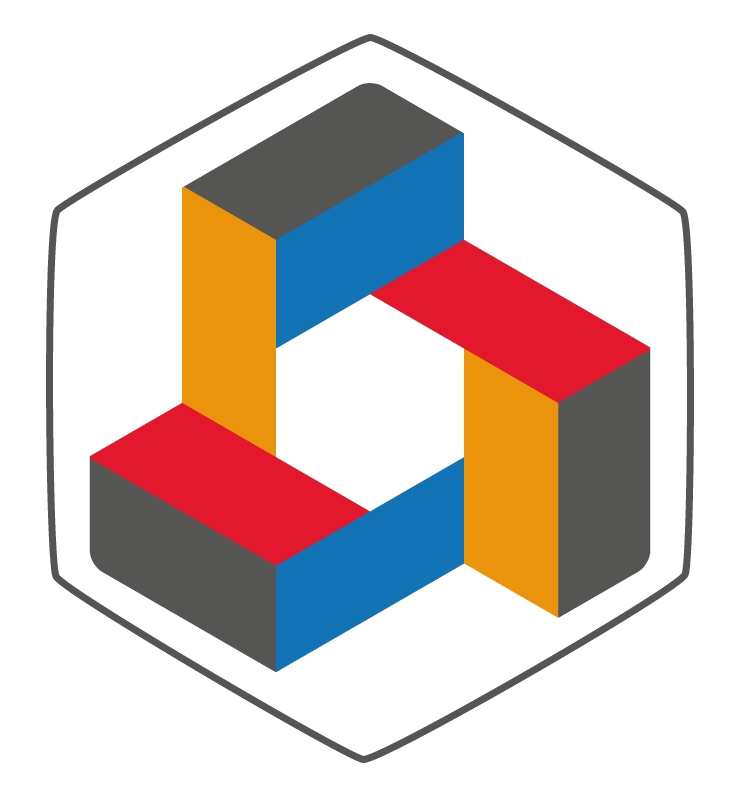
\includegraphics[scale=0.06]{../../logo/logo_lirmm.png}}
\fancyhead[C]{Rapport de Présentation - LIRMM - SuperBeeLive}
\fancyhead[R]{\includegraphics[scale=0.03]{../../logo/logo_polytech.png} \includegraphics[scale=0.3]{../../logo/logo_se.jpg}}
\fancyfoot[L]{\small Olivia SERENELLI-PESIN\normalsize}
\fancyfoot[C]{\includegraphics[scale=0.04]{../../logo/logo_superbeelive.png}}
\fancyfoot[R]{\thepage/\pageref{LastPage}}
\renewcommand{\footrulewidth}{0pt}
\renewcommand{\headrulewidth}{0.4pt}


\makeatletter
\let\ps@plain=\ps@fancy
\makeatother

\begin{document}

\begin{titlepage}
    \begin{center}
        \textsc{\LARGE Polytech Montpellier}\\
        \textsc{\Large Rapport d'entreprise Semestre 5}
        
        \HRule \\[0.4cm]
        { \huge \bfseries LIRMM - Projet SuperBeeLive\\[0.4cm]}
        \HRule \\ 

                \emph{Apprentie :} SERENELLI-PESIN Olivia
                \emph{Tutrice Académique :}Mme. DONADIEU Karen \\
                \emph{Maître d'Apprentissage :}M. DRUON Sébastien \\
    \end{center}
\end{sffamily}
\clearpage
\newpage

\title{Présentation de l'entreprise}

\subtitle{L'entreprise : le LIRMM}

Mon apprentissage en Système Embarqué s'inscrit dans un contexte de Recherche. Etant embauchée par l'Université 
de Montpellier, je travaille au LIRMM (Laboratoire d'Informatique, de Robotique et de Microélectronique de Montpellier) 
au sein de l'équipe EXPLORE, spécialisée dans la conception de robot pour l'exploration sous marine. \\
Plus précisement, j'ai été affectée au projet SuperBeeLive en tant qu'ingénieure de recherche afin de seconder M. Druon, 
mon maître d'apprentissage, dans les diverses tâches qu'il est amené à réaliser dans ce projet. \\

Le LIRMM est un laboratoire de recherche dépendant de l'Université de Montpellier et du Centre National de la Recherche 
Scientifique. Il est situé sur le Campus Saint-Priest de l'UM.
Il contient trois départements scientifiques : 
\begin{itemize}
    \item Informatique
    \item Microélectronique
    \item Robotique
\end{itemize} 

Le département informatique s'étend des mathématiques à la recherche appliquée : algorithmique des graphes, bioinformatique,
cryptographie, réseaux, bnase de données et système d'information, génie logiciel, intelligence artificielle, interaction homme-machine.
Le département microélectronique s'interesse aux domaines de la conception et du test de systèmes intéfrés et microsysèmes.
Enfin, le département Robotique va s'intéreseer aux problématiques de synthèse, de supervision et de gestion des systèmes dynamiques
complexes et de navigation, localisation et de pilotage de véhicules autnomes présents ou distants. 


Ainsi, mon lieu de travail principal est au LIRMM, mais je suis amenée à me déplacer à l'antenne du laboratoire à l'IUT de Béziers, 
mais aussi au CNRS où se trouve notre matériel de test pour le projet. 


Chiffres / organigramme / nombre de publication etc. 


\subtitle{Le projet SuperBeeLive}

La santé et le développement des abeilles sont aujourd’hui des questions de plus en plus étudiées. Les bouleversements
majeurs de notre planète et de l’activité humaine se traduisant par une augmentation alarmante de la mortalité
des colonies et une chute de la production du miel dans nos pays développés, il est urgent de se préoccuper de leur futur. 
La situation des abeilles domestiques alerte le pouvoir public sur l’accélération de la dégradation de la biodiversité des 
pollinisateurs domestiques et sauvages, et de la flore qui en dépend. Ces dégâts sont dûs, entre autres, à l’apparition 
et la prolifération d’espèces invasives pour les abeilles, provoquant maladies et détériorations. \\ 

Le projet consiste en la structuration de plusieurs collaborations existantes ou nouvelles autour du développement 
d’une ruche plate instrumentée destinée au monitorage détaillé de la santé de l’abeille et des écosystèmes. Son but est de
pouvoir répondre à des questions clé, notamment autour des mécanismes physiopathologiques et des maladies chroniques 
dûes aux parasites ainsi qu’aux altérations de l’écosystèmes et des qualités nutritives des produits des ruches. \\
Répondre à ces questions permettra de regrouper différentes solutions technologiques systèmatiques, 
automatiques et non-invasives à la collection de données usuelles déterminantes dans chacun des thèmes abordés.
Les différents travaux déjà effectués autour de ce sujet ne visaient qu’un seul type de problème à la fois, 
ne permettant pas une vision globale des difficultés rencontrées par les abeilles. Notre but est de réunir les différentes
données qui peuvent être utilisés pour étudier l’influence des éléments et événements extérieurs sur leur santé et leur cadre de vie.\\

Concrètement, l'équipe de SuperBeeLive va concevoir une ruche plate \footnote{Voir figures \ref{rpz_ruche} et \ref{photo_rucher}} afin d'y mettre 
en place plusieurs type  de capteurs (hygrométrie, vibrations, température interne et externe, etc) ainsi que des caméras qui filmeront 
l'intérieur et l'extérieur de la ruche. \\

Dans un premier temps, cette instrumentation nous permettra d'observer en temps réel la ruche et ses habitantes : 
les caméras nous donnerons une vision globale de ce qu'il s'y passe, aussi bien en intérieur pour observer leur 
comportement et tenter de repérer des parasites comme le varoa \footnote{Voir bibliographie \cite{ref11}}, 
qu'en extérieur pour y voir les dangers comme le frelon asiatique \footnote{Voir bibliographie \cite{ref12}}.
Couplée aux donnés récoltées à l'aide de la carte électronique et ses capteurs installés au centre de la ruche plate, 
nous pourrons avoir une vision complète et détaillée des événements et leur répercutions ponctuant la vie d'une colonie,
de sa naissance à sa mort. \\
Ces observations ont pour but d'être enregistrée, sauvegardées et commentées par les biologistes afin de construire une base
de donnée contenant plusieurs types de comportements reconnus comme le refroidissement de la ruche, les danses frétillante \footnote{Voir bibliographie \cite{ref10}}, 
etc.  
\\
Dans un second temps, cette base de donnée pourra être utilisée afin de créer des algorithmes repérant ces différents comportements
de manière automatisée. Cela nous permettrait, en plus d'avoir des données complètes, d'en avoir leur analyse en 
temps réel. Ces informations seront diffusées de deux façons. D'abord, elles seront partagées pour être étudiées par d'autres scientifiques, 
notamment les collaborateurs du projet SuperBeeLive. Le projet se veut aussi éducatif : une vitrine Web accessible au public 
sera créée présentant une ruche, ses données numériques et les vidéos commentées en direct par les algorithmes. \\


Ainsi, les ruches plates de SuperBeeLive permettront de fournir des données cruciales pour des futures recherches sur les 
abeilles. En plus, elles informeront le grand public sur leur importance et aux risques liées à nos activités humaines pour 
cette espèce et la biodiversité. 


\subtitle{L'équipe Superbeelive}
Le projet étant dans le domaine de la biologie, celui-ci est réalisé par plusieurs laboratoires de recherches. 
Les deux laboratoires porteurs du projets sont l'IBMM, L'institut des Biomolécules Max Mousseron avec Matthieu Rousset
et le CNRS, Centre National de la Recherche Scientifique avec Jean-Baptiste THUBAUD. On y retrouve également le LMGC, Laboratoire
de Mécanique et Génie Civil où sont réalisés les prototypes de la ruche plate et le LIRMM. 
En plus des laboratoires de recherches, une composante étudiante participe aussi au projet : l'IUT de Béziers, avec comme représentant
Philipe PUJAS, qui mettent à contribution les étudiants via des projets. Enfin, des partenaires internationnaux participent également :
l'Université de Wageningen. 
Le schéma suivant représente l'organigramme du projet avec le noms des personnes avec qui je travaille. \ref{orga_sbl}

\begin{figure}[!h]
    \centering 
    \includegraphics[scale=0.3]{}
    \label{orga_sbl}
\end{figure}

Au cours de mes missions, j'ai été et serai amenée à rencontrer tous les participants du projet, mais surtout les biologistes.
Le LIRMMM executant les parties techniques (gestion du réseau et des données, gestion des caméras, des capteurs et réalisation
des outils et algorithme d'analyse), nous devons questionner les biologistes sur les diverses contraintes autours des abeilles et 
de leur environnement afin d'adapter la ruche plate et mettre en place les meilleures installation pour nos mesures. 


\title{Mes missions}
Présentation globale des missions passées et à venir 
PAS UN RAPPORT TECHNIQUE DE STAGE --> reflexion à long terme sur mon immersion, implication et évolution dans l'entreprise
Compréhension globale de l'espace de travail 

Au vu du sujet du projet dans lequel je suis impliqué et de la taille de l'équipe pour le réaliser, j'ai été recrutée afin de réaliser 
un certains nombres de tâches variées. 
Ces tâches se répartissent dans plusieurs domaines, de l'électronique à la gestion de projet et humaine. 

Ainsi, nous travaillons principalement à deux sur toutes les parties du projet SuperBeeLive, mon maître d'apprentissage me
confiant la gestion de nos parties du projet. 

\subtitle{Création de la carte électronique}
La tâche principale de ma première année d'apprentissage est la création des cartes électroniques qui seront inserées dans 
les cadres du rucher. 
Notre but est de pouvoir récolter plusieurs types d'informations afin de les reporter le plus précisement possible sur une carte 
représentant le cadre et les valeurs récoltées. 
Ainsi, les biologistes pourront mettre en liens des informations telles que la températures ou l'hygrométrie avec les images 
prises par les caméras. 
Afin de réaliser cette carte, deux grandes étapes sont nécessaires : la maîtrise du microcontrôleur qui sera installé sur la 
carte avec les capteurs, et le dimensionnement de la carte avec le choix des capteurs. Une fois ces deux étapes faites, nous pourrons 
passer à la réalisation d'un premier prototype, idéalement pour l'été prochain. 

Le microcontrôleur que je vais devoir utiliser pour le contrôle de la carte est le STM32. Ce choix a été fait par M. Druon. 
Ainsi, il m'est demandé de connaître au mieux ce Microcontrôleur afin que lorsque nous serons amenés à le programmer et à l'utiliser, 
je sois la référence de l'équipe en ce qui le concerne. 
Pour cela j'ai, entre autre, plusieurs livres le concernant \footnote{Voir \cite{book1} et \cite{}}. 
De plus, nous désirons ne pas dépendre d'un IDE pour le développement avec la STM32. Il m'a été demandé de mettre en place 
une toolchain (chaine de compilation) pour Ubuntu et STM32 avec un guide d'utilisation. 
Avec ces outils, nous aurons une base solide pour travailler avec ce microcontroleur. 

Une fois ce premier travail réalisé, l'équipe sera opérationnelle pour le dimensionnement de la carte. Cette partie du travail
commencera par une étude des besoins et des ressources à disposition afin de choisir les capteurs en fonctions ce que nous pouvons
et devons faire. 
Les contraintes venant en grande partie de la place réservée pour les cartes électroniques dans les prototypes du rucher, mais 
aussi des conditions qu'imposent un tel milieu (activité des abeilles, température...). 
Plusieurs étapes viendront consituer ce dimensionnement, comme des tests avec un petit nombre de capteurs avant de concevoir la
première carte électronique. 

\subtitle{Développement d'un logiciel d'annotation pour les biologistes}
L'une des finalités du projet SuperBeeLive est d'avoir un ou plusieurs algorithmes capables de reconnaître automatiquement 
des comportements des abeilles, comme leur dances, des regroupements, ou des messages qu'elles se transmettent de diverses manières.
Ainsi, afin de pouvoir alimenter les bases de données permettant d'arriver à de tels algorithmes, il est nécessaire d'avoir 
déjà des vidéos annotées avec les informations permettant de repérer les dits comportements. 
Afin de faciliter cette tâche, qui sera surtout réalisée par les biologistes, ma première mission dans leur équipe lors de mon 
stage de fin de DUT avait été de développer un logiciel d'annotation vidéo. Ce logiciel, correspondant aux besoins exacts des 
biologiste, permettra, une fois fini, d'annoter avec des figures disposables sur les vidéos, des textes et des tags permettant de
classer et retrouver les vidéos facilement, d'avoir une base de donnée précise et utilisable pour que les roboticiens (LIRMM) puissent
l'exploiter. 

Aujourd'hui, toute la partie graphique a été réalisée \footnote{Voir les figures \ref{}}, et nous avons déjà une interface bien 
définie \footnote{Voir la figure \ref{} PLAN DE L'INTERFACE AVEC DESSIN/BLOC}
Il reste encore du travail concernant le lien entre les capteurs, les caméras etc et l'interface ainsi que la sauvegarde
des données sur nos serveurs. 

Le développement de ce logiciel, même si bien avancé, n'est pas encore fini et a pour projet de l'être d'ici la fin de l'année 2020. 
J'ai donc comme mission de finir son développement avec mon maître d'apprentissage et surtout de le mettre à jour en corrigeant les 
possibles bugs et en prenant en compte les retours utilisateurs lorsque celui-ci sera disponible. 


\subtitle{Mise en place et gestion du réseau du rucher et de ces équipements}
Nous travaillons sur une ruche plate expérimentale, celle-ci est installée au CNRS et il a été tiré deux fibre afin d'avoir 
une connexion internet rapide et assez conséquente par rapport aux données qui sont prévues d'être enregistrées et envoyées. 
En effet, les biologistes ont exprimé le besoin de sauvegarder la casi intégralités des vidéos et données numériques des capteurs
de la naissance à la mort de la ruche, ce qui serait une première en terme de données autours des abeilles. Seulement, 
une telle sauvegarde de données nécessite un réseau solide sur place mais aussi et surtout un serveur avec une capacité 
de stockage assez conséquente afin de pouvoir supporter un tel flot de donnée (de l'ordre du petaoctet). 
Le dimensionnement du serveur a été fait et sera confirmé par l'équipe informatique du LIRMM, mais une connaissance 
de l'architecture et de la configuration du serveur dans l'équipe directement est primmordiale pour pouvoir travailler dessus
et gérer directement la sauvegarde des données. 
Il m'a donc été demandé de suivre cette installation et d'avoir une veille technologique concernant le serveur et l'architecture
utilisées. 

Enfin, quelques équipements réseau ont été et vont être installés au rucher \foonote{Voir figure \ref{}}. 
Leur mise en place et gestion m'ont également été confiés.

\begin{figure}
    \centering
    \includegraphics[scale=0.7]{}
    \caption{Réseau du rucher}
    \label{reseau_rucher}
\end{figure} 

\subtitle{Gestion de projet étudiants}
Afin d'avoir une composante gestion
Actuellement : 6 groupes de projets RT1 
A venir : stage M1 robotique


\title{Le rapport au DDRS de l'entreprise}
Partie DDRS : Développement durable et Responsabilité Sociétale (DD-RS) 

Répondre aux questions suivantes : 
- Position de l'entreprise vis à vis des enjeux du DD RS ? 
Levier qui motivent l'intérêt de l'entrepmrse pour le DD RS ? 
Organisation mise en place popur répondre à ces questions ? 
Actions mises en oeuvre ? 








\end{document}  
